% Geometry, font
\documentclass[12pt, letter]{article}
\usepackage[margin=0.8in]{geometry}
\usepackage[T1]{fontenc}
\usepackage{fourier}
\usepackage{titling}
\setlength{\droptitle}{-5em} 
\usepackage[parfill]{parskip}
\usepackage{graphicx}
\graphicspath{{imgs/}}
\usepackage{hyperref}

% Math stuff
\usepackage{amssymb}
\usepackage{amsmath}
\usepackage{bm}

% Code Highlighting
\usepackage{minted}
\usemintedstyle{solarizedlight}

\author{Zach Neveu}
\title{ Day 2: Frequency Transforms, Filtering }

\begin{document}
\maketitle

\section{Filtering}%
\label{sec:filtering}

\begin{figure}[h]
	\centering
	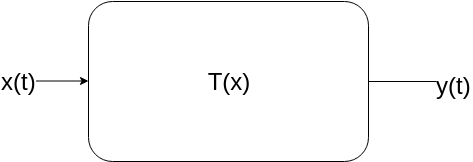
\includegraphics[width=0.8\textwidth]{lin-sys}
	\caption{Generic System}
	\label{fig:lin-sys}
\end{figure}
\begin{itemize}
	\item Traditional DSP System: $x(n) \to T[x(n)] \to y(n)$
	\item $T[x(n)] = x^2(n-1)$ 
	\item Bold number in sequence is where $n=0$ by convention
	\item $x(n) = \{-1, \mathbf{0}, 1, 2, 3\}$
	\item $y(n) = \{\mathbf{1}, 0, 1, 4, 9\}$ delayed by 1
	\item Superposition (proves linearity):
	\item $x(n) = a_1x_1(n)+a_2x_2(n) \to T[x(n)] = a_1T[x_1(n)]+a_2T[x_2(n)]$ 
	\item $y(n) = a^2 x(n) \to $ linear
	\item $y(n) = ax^2(n) \to$ non-linear
	\item $y(n) = nx(n) \to$ time-varying
	\item $y(n) = x(-n) \to$ time-varying
	\item if $y(n+k) = T(x(n+k))$ then time invariant
	\item General linear system: $y(n) = - \sum_{k=1}^{N} a_ky(n-k) + \sum_{k=0}^{M} b_kx(n-k)$
	\item This is just like a discrete convolution! No wonder this is so important to DSP\ldots
	\item First term is recursive: goes from last output back to Nth previous
	\item Second term is non-recursive; depends only on past M inputs
	\item FIR filters have only second term
	\item IIR filters have first term
	\item General system equation can be distilled into $x(n)*h(n)$ using the convolution
\end{itemize}

\section{Example Problems}%
\label{sec:example_problems}
\begin{itemize}
	\item Linear system with coeffs $a_k = 0, b_0 = 1, b_1 = 2, b_2=1, b_i=0, i\ge 3$
	\item $y(x) = x(n-1)+2x(n-2)+x(n-3)$ 
	\item $x(n) = \{\ldots,0, \mathbf{1}, 0,\ldots\}$
	\item $y(n) = \{\ldots,0,1,2,1,0,\ldots\} \to$ Impulse Response!
\end{itemize}

\section{More Notes}%
\label{sec:more_notes}

\begin{itemize}
	\item Fourier vs. Z transform
	\item Z transform is generalized Fourier transform
	\item Can use Z transform instead of Fourier
	\item Equal when:
	\item $X(f) = X(z)_{z=e^{j_2\pi f}}$
	\item Time domain: $y(n) = h(n)x(n)$
	 \item z-domain: $Y(Z) = H(Z)X(Z)$
	\item $H(Z) = \sum_{n=-\infty}^{\infty} h(n)z^{-n} = \frac{Y(Z)}{X(Z)}  = \frac{\sum_{k=0}^{M} b_kz^{-k}}{1+\sum_{k=0}^{N} a_kz^{-k}}$
\end{itemize}

\section{Time-Frequency Analysis}%
\begin{itemize}
	\item Spectrograms - STFT at each time window
	\item DFT - Discrete Fourier Transform
	\item DFT: $X(k) = \sum_{n=0}^{N-1} x(n)e^{j_\frac{2\pi}{N}kn}$
	\item STFT: $x(n,k) = \sum_{m=-\infty}^{\infty} x(m)w(m-n)e^{-j_\frac{2\pi}{N}kn}$
	\item New signal for STFT: $\hat{x}(n) = x(m)*w(m-n)$
	\item $w(m-n)$ is window function
	\item Multiplication in time domain is convolution in freq domain, so window function will be convolved with signal in freq. domain
	\item Ideal $W(F)$ is a dirac delta, so ideal  $w(t)$ is a sinc function
	\item sinc has infinite time, so window is infinite, so not actually stft
	\item Must compromise and chop the sinc function
	\item Look for 3dB point of sinc, as well as main lobe width.
	\item Types of window functions: Rect, Bartlett, Hann, Hamming
	\item Rectangular tightest main lobe, but most leakage. High resolution, but lots of noise/ripples
	\item Hann most commonly used
	\item Important spectrogram params: block size (B) and hop size (S)
	\item Block size: how many samples in each calculation? How big is window?
	\item Hop size: how far to jump forward before calculating next frame?
	\item Large block size - low time resolution, small block size - low frequency resolution
	\item Hop size: small hop size - very smooth over time, large hop size - less smooth
\end{itemize}

\section{Wavelet Transform}%
\label{sec:wavelet_transform}
\begin{itemize}
	\item $X(s,\tau) = \int_t x(t)\phi^*_{s,\tau}(t)dt$
	\item Similar to Fourier transform, $s,\tau \to F$
	\item $s \to $ scaling
	\item $\tau \to$ transformation
	\item Idea: start with a simple wavelet pulse function. Shift it to infinite positions in time domain, stretch it to shift in frequency domain.
	\item Essentially, STFT makes a grid in time/freq, wavelet creates a wavelet for each square and measures correlation
	\item Low frequencies have longer window length, high frequencies have shorter window lengths!
\end{itemize}


\end{document}
